\def\module{MATH40005A Probability}
\def\lecturer{Professor Almut Veraart}
\def\term{Autumn 2023}
\def\cover{
$$
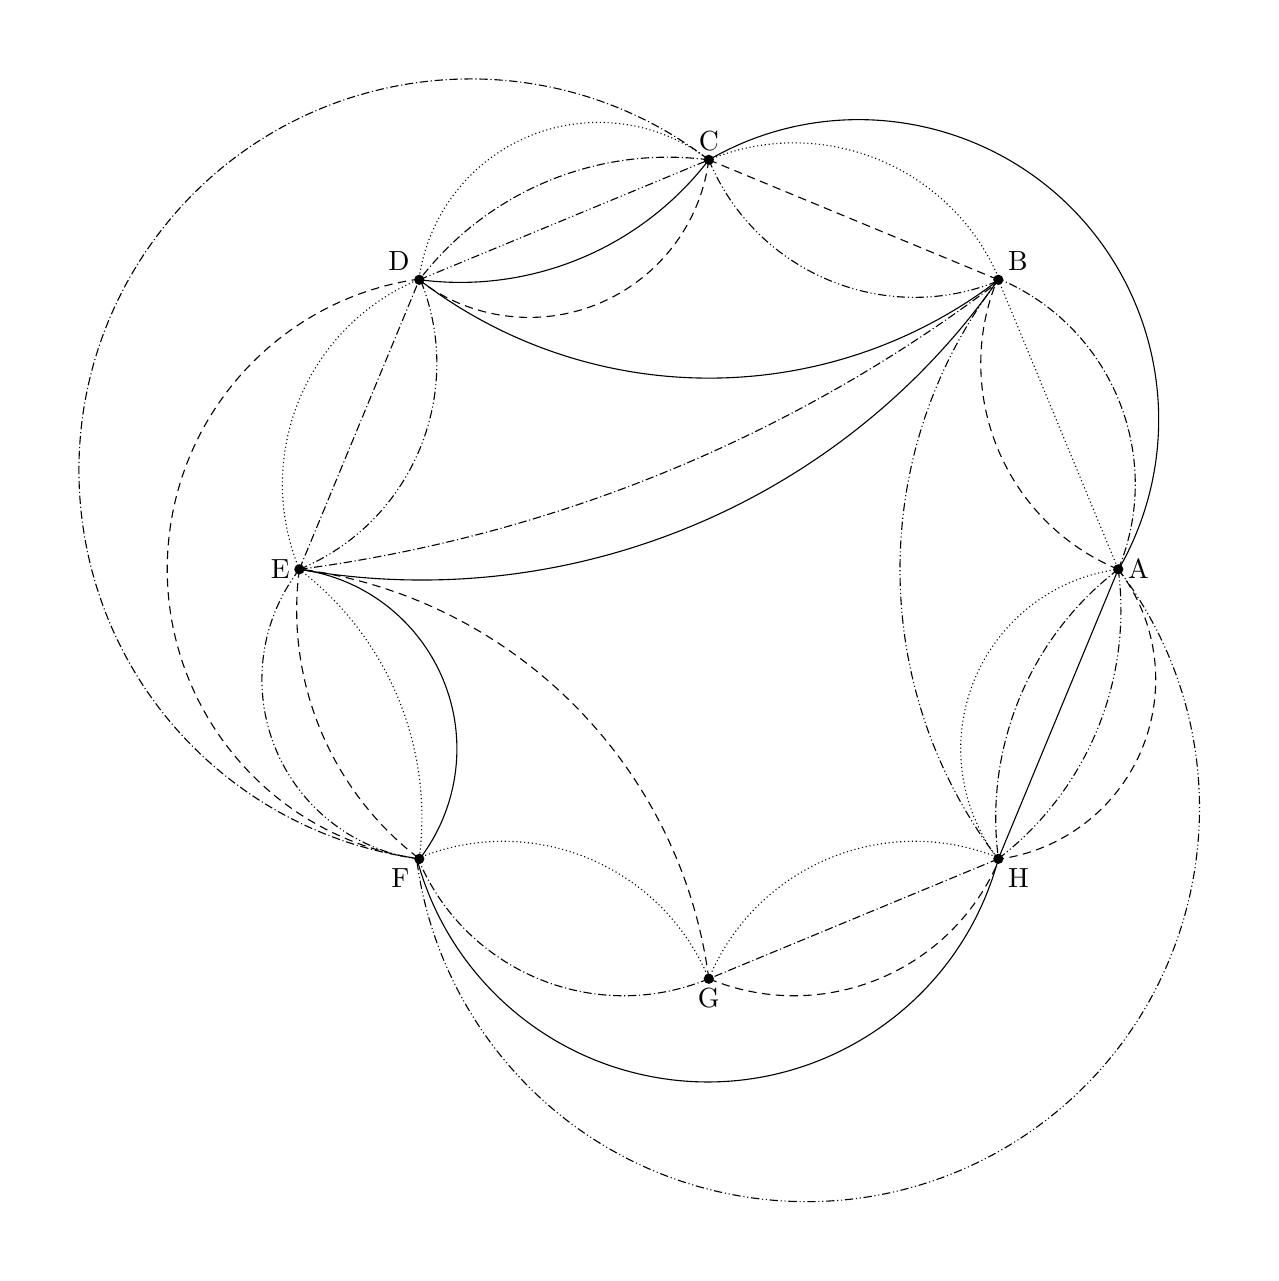
\begin{tikzpicture}[scale=1.3]
    \draw[black] (4,0) -- ({2*sqrt(2)},{-2*sqrt(2)});
    \draw[black] (0,4) arc (-37.5:-97.5:3.06);
    \draw[black] (-4,0) arc (82.5:-37.5:1.77);
    \draw[black] (0,4) arc (120:-30:2.93);
    \draw[black] ({2*sqrt(2)},{-2*sqrt(2)}) arc (-15:-165:2.94);
    \draw[black] ({-2*sqrt(2)},{2*sqrt(2)}) arc (232.5:307.5:4.65);
    \draw[black] (-4,0) arc (-100:-34.8:6.875);
    
    \draw[black, densely dotted] ({2*sqrt(2)},{2*sqrt(2)}) -- (4,0);
    \draw[black, densely dotted] (-4,0) arc (52.5:-7.5:3.06);
    \draw[black, densely dotted] (0,4) arc (112.5:22.5:2.175);
    \draw[black, densely dotted] (0,-4) arc (22.5:112.5:2.175);
    \draw[black, densely dotted] (0,-4) arc (157.5:67.5:2.175);
    \draw[black, densely dotted] (-4,0) arc(202.5:112.5:2.17);
    \draw[black, densely dotted] (0,4) arc (52.5:172.5:1.77);
    \draw[black, densely dotted] (4,0) arc (97.5:217.5:1.77);
    
    \draw[black, densely dashed] (0,4) -- ({2*sqrt(2)},{2*sqrt(2)});
    \draw[black, densely dashed] (-4,0) arc (172.5:232.5:3.06);
    \draw[black, densely dashed] (4,0) arc (247.5:157.5:2.175);
    \draw[black, densely dashed] (0,-4) arc (-112.5:-22.5:2.175);
    \draw[black, densely dashed] (4,0) arc (37.5:-82.5:1.77);
    \draw[black, densely dashed] (0,4) arc (-7.5:-127.5:1.77);
    \draw[black, densely dashed] ({-2*sqrt(2)},{-2*sqrt(2)}) arc (-98:-262:2.86);
    \draw[black, densely dashed] (0,-4) arc (7.5:82.5:4.65);
    
    \draw[black, densely dashdotted] ({2*sqrt(2)},{-2*sqrt(2)}) -- (0,-4);
    \draw[black, densely dashdotted] (-4,0) -- ({-2*sqrt(2)},{2*sqrt(2)});
    \draw[black, densely dashdotted] (0,4) arc (82.5:142.5:3.06);
    \draw[black, densely dashdotted] (4,0) arc (127.5:187.5:3.06);
    \draw[black, densely dashdotted] (4,0) arc (-22.5:67.5:2.175);
    \draw[black, densely dashdotted] (0,-4) arc (-67.5:-157.5:2.175);
    \draw[black, densely dashdotted] (0,4) arc (52.5:262.5:3.825);
    \draw[black, densely dashdotted] (-4,0) arc (-82.5:-52.8:14.4);
    
    \draw[black, densely dashdotdotted] ({-2*sqrt(2)},{2*sqrt(2)}) -- (0,4);
    \draw[black, densely dashdotdotted] (4,0) arc (7.5:-52.5:3.06);
    \draw[black, densely dashdotdotted] (0,4) arc (202.5:292.5:2.175);
    \draw[black, densely dashdotdotted] (-4,0) arc (-67.5:22.5:2.175);
    \draw[black, densely dashdotdotted] (-4,0) arc (142.5:262.5:1.77);
    \draw[black, densely dashdotdotted] (4,0) arc (37.5:-172.5:3.84);
    \draw[black, densely dashdotdotted] ({2*sqrt(2)},{2*sqrt(2)}) arc (142.5:217.5:4.65);
    
    \fill (4,0) circle (0.05) node[right]{A};
    \fill ({2*sqrt(2)},{2*sqrt(2)}) circle (0.05) node[above right]{B};
    \fill (0,4) circle (0.05) node[above]{C};
    \fill ({-2*sqrt(2)},{2*sqrt(2)}) circle (0.05) node[above left]{D};
    \fill (-4,0) circle (0.05) node[left]{E};
    \fill ({-2*sqrt(2)},{-2*sqrt(2)}) circle (0.05) node[below left]{F};
    \fill (0,-4) circle (0.05) node[below]{G};
    \fill ({2*sqrt(2)},{-2*sqrt(2)}) circle (0.05) node[below right]{H};
\end{tikzpicture}
$$

\begin{center}
    A minimum vertex 5-Venn diagram.
\end{center}
}
\def\syllabus{Basic set theory and combinatorics, Kolmogorov probability axioms, DRVs, CRVs, Transformations, Expectaction, Variance, Multivariate calculus, Joint Distributions, LOTUS, pgfs, mgfs, conditional distribution}
\def\thm{subsection}

\input{../style/header}

\begin{document}

\input{../style/cover}

\section{Introduction}

\lecture{1}{Monday}{30/10/2023}

The following are complementary reading for the course.
\begin{itemize}
\item G. Grimmett and D. J. A. Welsh, Probability: An Introduction, 1986
\item J. K. Blitzstein and J. Hwang, Introduction to Probability, 2019
\item D. F. Anderson et al, Introduction to Probability, 2018
\item S. M. Ross, Introduction to Pro ability Models, 2014
\end{itemize}

\begin{notation*}
    Denote the natural numbers by $\NN = \{1,2,...\}$ and define $\NN_0 := \NN \cup \{0\}$. Moreover, denote the integers by $\ZZ = \{...,-2,-1,0,1,2,...\}$ and the reals by $\RR$. For real numbers $a < b$ write $[a,b]$ and $(a,b)$ for closed and open intervals respectively.
\end{notation*}

\section{Sample spaces and interpretations of probability}

\subsection{Sample spaces and set theory}

\begin{definition}
    The \textbf{sample space} $\Omega$ is the set of all possible outcomes of an experiment. An element of the sample space $\omega \in \Omega$ is a \textbf{sample point}.
\end{definition}

\begin{examples}
    When flipping a coin $\Omega  = \{H,T\}$. When rolling a standard die $\Omega = \{1,2,3,4,5,6\}$.
\end{examples}

\begin{definition}
    Subsets of $\Omega$ are collections of sample points and called \textbf{events}.
\end{definition}

Suppose events $A,B\subseteq\Omega$:
\begin{itemize}
    \item $A\cup B$ is the event that $A$ or $B$ or both occur.
    \item $A\cap B$ is the event that $A$ and $B$ both occur.
    \item $A^c = \bar{A}$ is the event that occurs iff $A$ does not occur.
\end{itemize}


Let $\III$ be a general index set with $A_i \subseteq\Omega,\; \forall i \in\III$ and $B \subseteq \Omega$. The following identities hold.
\[
\left( \bigcup_{i\in\III}A_i \right)^c = \bigcap_{i\in\III}A_i^c \textcolor{black}{,} \quad
\left( \bigcap_{i\in\III}A_i \right)^c = \bigcup_{i\in\III}A_i^c \textcolor{black}{,} \qquad
B \cap \left( \bigcup_{i\in\III}A_i \right) = \bigcap_{i\in\III}(A_i\cup B) \textcolor{black}{,} \quad
B \cup \left( \bigcap_{i\in\III}A_i \right) = \bigcup_{i\in\III}(A_i\cap B) \textcolor{black}{.}
\]
These are \textbf{De Morgan's Laws} and \textbf{Distributivity} respectively.

\lecture{2}{Tuesday}{31/10/2023}

\subsection{Interpretation of probability}
\begin{definition}
    The \textbf{Cardinality} of a set, denoted $\text{card}(A)$ or $|A|$ is the number of elements in the set $A$.
\end{definition}

\begin{definition}
    Two sets have the same cardinality iff there exists a bijection between the them.
\end{definition}

\begin{definition}
    $A$ is \textbf{finite} if it has as finite numbers of elements, $A$ is \textbf{countably infinite} if there exists a bijection $f: A \to \NN$, $A$ if \textbf{countable} if it is finite or countable infinite, $A$ is \textbf{uncountable} or \textbf{uncountable infinite} if it isn't countable.
\end{definition}

Samples spaces can be countable or uncountable.

\begin{definition}[Naive probability]
    Suppose $|A| < \infty$ and we want to assign a probability to $A \subseteq \Omega$.
    \[
    \PP_{Naive}(A) := \frac{|A|}{|\Omega|} \implies \PP(A^c) = 1 - \PP(A)  \textcolor{black}{.}
    \]
    This Naive example does not consider when $|A|$ is infinite but of finite area.
\end{definition}
\begin{example}
    Let $\Omega = \{(x,y) \in \RR^2, x^2+y^2=1\}$ and $A\subseteq\Omega$. Define: 
    \[
    \PP(A) := \frac{\text{area of } A}{\text{area of } \Omega}
    \]
    In the case where $A = \{(x,y) \in \RR^2, x^2+y^2=0.5^2\}$ we have $\PP(A) = 0.25$
\end{example}
\begin{remark}
    For classical / naive probability we require $|\Omega| < \infty$ or the ``area" of $\Omega$ be finite. 
\end{remark}

\begin{definition}[Limiting frequency]
    Consider $n_{total}$ repetitions of an experiment and $n_A$ the number of time $A$ occurs.
    \[\PP(A) := \lim_{n_{total} \to \infty} \frac{n_A}{n_{total}}\]
    Unfortunately, $n_{total} \to \infty$ is often hard to conceive with finite representations not necessarily being representative.
\end{definition}

\begin{definition}[Subjective probability]
    For an event $A$ assign the probability $\PP(A)$ based on our own personal beliefs. The subjective probability need not be the same for different individuals, and despite its appearance it remains a valid interpretation of probability.
\end{definition}

\begin{remark}
    All three interpretations of probability depend of assumptions about the experiment.
\end{remark}

\lecture{3}{Friday}{03/11/2023}

\section{Counting}
\subsection{Multiplication principle}
Computing naive probabilities often requires some combinatorics.

\begin{definition}[Multiplication  principle]
    If we perform an experiment $A$ that has $a$ possible outcomes and an experiment $B$ with $b$ possible outcomes (in any order) then the number of outcomes of the  \textbf{compound experiment} will be $ab$.
\end{definition}

\begin{remark}
    When dealing with repetitions of the same experiment (with sample space $\Omega$, the sample space is given by the Cartesian product of the individual samples spaces.
    \[
        \Omega_1 \times \Omega_2 \times \cdots \times \Omega_n :=  \{(\omega_1,\omega_2,\ldots,\omega_n): \omega_i \in \Omega_i\}\textcolor{black}{.}
    \]
    The cardinality of this samples space follows from the multiplication principle.
\end{remark}

\subsection{Power sets}
\begingroup\belowdisplayskip=-10pt
    \begin{definition}[Power Set]
        Given a set $A$ its \textbf{power set} is defined as:
        \[
            \PPP(A) := \{X,X\subseteq A\}\textcolor{black}{.}
        \]
    \end{definition}
\endgroup

\begin{theorem}
    If $A$ is a finite set, $|\PPP(A)|=2^{|A|}$.
\end{theorem}

\subsection{Combinatorial coefficients}

\begingroup\belowdisplayskip=-0pt
    \begin{definition}[Factorial]
        Let $n\in\NN$ the \textbf{factorial} of $n$ is defined as:
        \[
        n! := \prod_{i=1}^ni\textcolor{black}{.}
        \]
    \end{definition}
\endgroup

\begingroup\belowdisplayskip=-10pt
    \begin{definition}[Descending factorial]
        Let $k,n\in\NN$ with $k\leq n$ the \textbf{descending factorial} denoted $(n)_k$ is defined as:
        \[
        (n)_k := n(n-1)\ldots(n-k+1) = \prod_{i=0}^{k-1}(n-i) = \prod_{j=n-k+1}^{n}j = \frac{n!}{(n-k)!}\textcolor{black}{.}
        \]
    \end{definition}
\endgroup

\begingroup\belowdisplayskip=-10pt
    \begin{definition}[Binomial coefficient]
        Let $k,n\in\NN\cup \{0\}$ the \textbf{binomial coefficient} is the number of subsets of size $k$ of a set $n$:
        \[
        \binom{n}{k} := 
        \begin{dcases}
            \frac{n(n-1)\ldots(n-(k-1))}{k!} = \frac{(n)_k}{k!} = \frac{n!}{(n-k)!k!} & \textcolor{black}{\text{if }} k\leq n \\
            \omit\hfil$0$\hfil & \textcolor{black}{\text{otherwise.}}
        \end{dcases}
        \]
    \end{definition}
\endgroup

\subsection{Sampling with and without replacement}
``Definitions" given in the context of drawing balls from an urn, $S=\{1,2,\ldots,n\}$.
\begin{definition}[Ordered sampling with replacement]
    Take out a ball from $S$, note its number, put it back; repeat this $k$ times. The sample space for this experiment is $\Omega = S^k$.
\begin{definition}[Ordered sampling without replacement]
    Take out a ball form $S$, note its number but \textbf{do not} put it back; repeat $k<n$ times.
\end{definition}
\end{definition}
\end{document}